\documentclass[12pt,a4paper,parskip=half,listof=totoc]{scrreprt}
% Dokumenteninformationen
\title{Asynchrones Programmieren in Clojure}
\author{Vincent Elliott Wagner, Tobias Schwalm}

%export author and title to use later
\makeatletter
\let\thetitle\@title
\let\theauthor\@author
\makeatother





\usepackage[utf8]{inputenc}
\usepackage[T1]{fontenc}
\usepackage{lmodern}

%\usepackage[scaled]{uarial}


%use serif font
\renewcommand*\familydefault{\rmdefault}
%use san serif font
%\renewcommand*\familydefault{\sfdefault}

% Farben festlegen
\usepackage{xcolor}
\definecolor{black}{rgb}{0.0,0.0,0.0}

% Packet für bessere Listen vorallem Kompakte
\usepackage{paralist}


% Bilder einfügen
\usepackage{graphicx}

% Bilder fest positionieren
\usepackage{float}

% Fußnotenzähler durchgängig
\usepackage{chngcntr}
%\counterwithout{footnote}{chapter}

\usepackage{perpage} %the perpage package
\MakePerPage{footnote} %the perpage package command



% Deutsche Übersetzungen automatisch eingefügter Worte
\usepackage[ngerman]{babel}

% Acronyme bzw. Abkürzungen
\usepackage[printonlyused]{acronym}




%\usepackage{relsize}
%\usepackage{xcolor}
%\renewcommand{\bflabel}[1]{#1\hfill}
\renewcommand{\bflabel}[1]{\normalfont{\normalsize{#1}}\hfill}
% kursiv long
\renewcommand*{\acffont}[1]{{\color{black}\itshape{#1}}}
\renewcommand*{\acfsfont}[1]{\textnormal{#1}}

% Subfigure
\usepackage{subfigure}

% Advanced tables
\usepackage{tabularx}

%\usepackage[perpage]{footmisc}

%package for odd pages check
%\usepackage{changepage}
%\strictpagecheck


\definecolor{listing_bg}{rgb}	{0.98,0.98,0.98}

% Listing package (Code,...)
\usepackage{listings}

\lstdefinelanguage{Clojure}
  {morekeywords={defn, defmacro, let, if, when, loop, recur},
    sensitive=false,
    morecomment=[l]{;;},
    morecomment=[s]{/*}{*/},
    morestring=[b]",
    ndkeywordstyle=\color{darkgray}\bfseries,
    identifierstyle=\color{black},
    sensitive=false,
    comment=[l]{//},
    morecomment=[s]{/*}{*/},
    commentstyle=\color{purple}\ttfamily,
    stringstyle=\color{red}\ttfamily,
    morestring=[b]',
    morestring=[b]"
  }

\lstdefinelanguage{JavaScript}{
  keywords={typeof, new, true, false, catch, function, return, null, catch, switch, var, if, in, while, do, else, case, break},
  keywordstyle=\color{blue}\bfseries,
  ndkeywords={class, export, boolean, throw, implements, import, this},
  ndkeywordstyle=\color{darkgray}\bfseries,
  identifierstyle=\color{black},
  sensitive=false,
  comment=[l]{//},
  morecomment=[s]{/*}{*/},
  commentstyle=\color{purple}\ttfamily,
  stringstyle=\color{red}\ttfamily,
  morestring=[b]',
  morestring=[b]"
}

\lstloadlanguages{Java}
\lstset{
	basicstyle			= \footnotesize,
	frame						= trLB, 							% Rahmen (right, bottom, left, top; uppercase: double frame)
	breaklines			= true, 							% Zeilenumbruch
	numbers					= left, 							% Zeilennummernformatierung: Schriftausrichtung
	numberstyle			= \tiny, 							% Zeilennummernformatierung: Schriftgroesse
	backgroundcolor	= \color{listing_bg}, % Hintergrundfarbe
	tabsize					= 2, 									% col1 = n+1, col2 = 2n+1
	extendedchars		= true 								% Sonderzeichen
}

% Verhindere unterstreichen von Titeln im Literaturverzeichnis
\usepackage[normalem]{ulem}

% Verwende biblatex um zusätzliche Zitatfunktionen zu ermöglichen
%\usepackage[style=alphabetic,hyperref=true,backend=bibtex8]{biblatex}
%\usepackage[autocite=footnote, style=authortitle-icomp, citestyle=authortitle-icomp, maxcitenames=1]{biblatex}
\usepackage[autocite=footnote, style=authortitle-icomp, citestyle=authortitle-icomp, maxcitenames=1]{biblatex}
\bibliography{Literaturverzeichnis}{\addcontentsline{toc}{chapter}{Literaturverzeichnis}}

\renewbibmacro*{cite:title}{%
  \printtext[bibhyperref]{%
    \printfield[citetitle]{labeltitle}%
    \setunit{\addcomma\space}%
    \printdate}}

%booleans und vergleiche
\usepackage{ifthen}



% Abkürzungen
\newcommand{\bzw}{\mbox{bzw.}}
\newcommand{\CA}{\textit{core.async}}



% Meta Information festlegen IMPORT LAST
\usepackage[
    pdftitle={Asynchrones Programmieren in Clojure mit Hilfe der Bibliothek core.async},
    pdfsubject={Asynchrones Programmieren in Clojure mit Hilfe der Bibliothek core.async},
    pdfauthor={\theauthor},
    pdfkeywords={Clojure, core.async, WS13/14}
]{hyperref}

%  Grafiken richtig verlinken
\usepackage[all]{hypcap}


% Links richtig färben
\hypersetup{
	linkcolor		= black,	% red 		Color for normal internal links. 
	anchorcolor		= black,	% black 	Color for anchor text. 
	citecolor		= black,	% green 	Color for bibliographical citations in text. 
	filecolor		= black,	% magenta	Color for URLs which open local files. 
	menucolor		= black,	% red 		Color for Acrobat menu items. 
	urlcolor		= black,	% cyan 		Color for linked URLs.
	colorlinks		= true		% Use colored text instead of a frame around it.
	}
	
%More Text Symbols bullets ...	
\usepackage{textcomp}

% Dicke horizontale Linien mit \Xhline{2\arrayrulewidth}
\usepackage{makecell}


\newcommand\footnoteref[1]{\protected@xdef\@thefnmark{\ref{#1}}\@footnotemark}

%Unterstreichen von allem möglichen
%\usepackage{ulem}

% Rotieren der Tabellen
%\usepackage{rotating}
% Trennung von Wörtern verhindern
\usepackage{hyphenat}
%Mathematiksymbole
\usepackage{amsmath}

	
	
%cannot be in another file
\usepackage{glossaries}
\makeglossaries
%\setcounter{secnumdepth}{5}

\begin{document}
% Titelseite einfügen
\maketitle
% Leere Seite nach Titelseite
\newpage
%\cleardoublepage

% Inhaltsverzeichnis
\pagenumbering{Roman}
\setcounter{page}{1}
%\phantomsection
%\addcontentsline{toc}{chapter}{Inhaltsverzeichnis}
%\tableofcontents
%\newpage

% Sichern der aktuellen Seitenzahl des Vorspanns
\newcounter{last_roman}
\setcounter{last_roman}{\value{page}}

% Kapitel
\pagenumbering{arabic}
\chapter{Asynchrones Programmieren in Clojure mit Hilfe der Bibliothek core.async}
\section{Einleitung}
Diese Ausarbeitung befasst sich mit \CA , einer Bibliothek zur asynchronen Programmierung in der Programmiersprache Clojure. Es werden zunächst die grundlegenden Begrifflichkeiten erklärt, andere State-of-the-Art Programmierparadigmen, Entwurfsmuster und Frameworks betrachtet und anschließend mit \CA\ verglichen. Anhand von Beispielen aus dem \acf{API} des Frameworks, wird der aktuelle Entwicklungsstand des noch im Alpha-Stadium befindlichen Frameworks gezeigt und dessen Potential bewertet.
\section{Technologien}
\subsection{Was bedeutet asynchrone Programmierung?}
Zu Beginn stellt sich die Frage nach der Erläuterung des Begriffs \textit{asynchrone Programmierung}. Betrachten wir eine imperative Programmiersprache ohne Multithreading, so lässt sich dieser Begriff leicht erklären. Eine Anwendung in einem imperativen Kontext hat ihren Entry-Point in der ersten Zeile des Programmcodes. Der Code wird streng sequentiell abgearbeitet. Jeder Befehl blockiert die Anwendung, solange bis seine Abarbeitung beendet ist. Dieses Verhalten einer Anwendung wird als \textit{synchrone} Abarbeitung einer Befehlsfolge bezeichnet. Der Nachteil ist hier, dass Wartezeiten zwischen Berechnungen entstehen. Lange Berechnungen reduzieren die Performance der Anwendung, da stets auf ihre Beendigung gewartet werden muss. Hier kommt \textit{asynchrone Programmierung} zum Tragen. Der Begriff beschreibt eine sequentielle Befehlsabarbeitung, bei der keine Wartezeit zwischen Berechnungen entsteht. Die Grundlage hierfür stellen ein nichtblockierendes I/O-Modell, welches im nächsten Kapitel erklärt wird, sowie diverse Programmierparadigmen dar.


\subsection{Blockierende und nichtblockierende \acs{I/O}}
\label{sec:nonblocking}Ein nichtblockierendes I/O-Modell ermöglicht die Verarbeitung von Befehlen bei zeitintensiven Berechnungen oder Datenbankabfragen ohne dass der Main-Thread der Anwendung blockiert wird. Es muss nicht auf das Ergebnis der Berechnung gewartet werden, bevor der nächste Befehl ausgeführt werden kann. Der Mechanismus kann beispielsweise mit Hilfe einer Ereignisschleife umgesetzt werden, die die Vorgänge in sogenannten Worker-Threads auslagert und nach Beendigung der Aufgaben die Callback-Funktionen aufruft, die im Main-Thread abgearbeitet werden (siehe Abb. \ref{fig:nonblocking}). Diese Technik nennt sich \acf{CPS} und wird im Kapitel \ref{sec:jscps} am Beispiel von JavaScript erklärt. Ein nichtblockierendes I/O-Modell stellt die Grundlage für asynchrone Programmierung dar.
\begin{figure}[H]
\centering
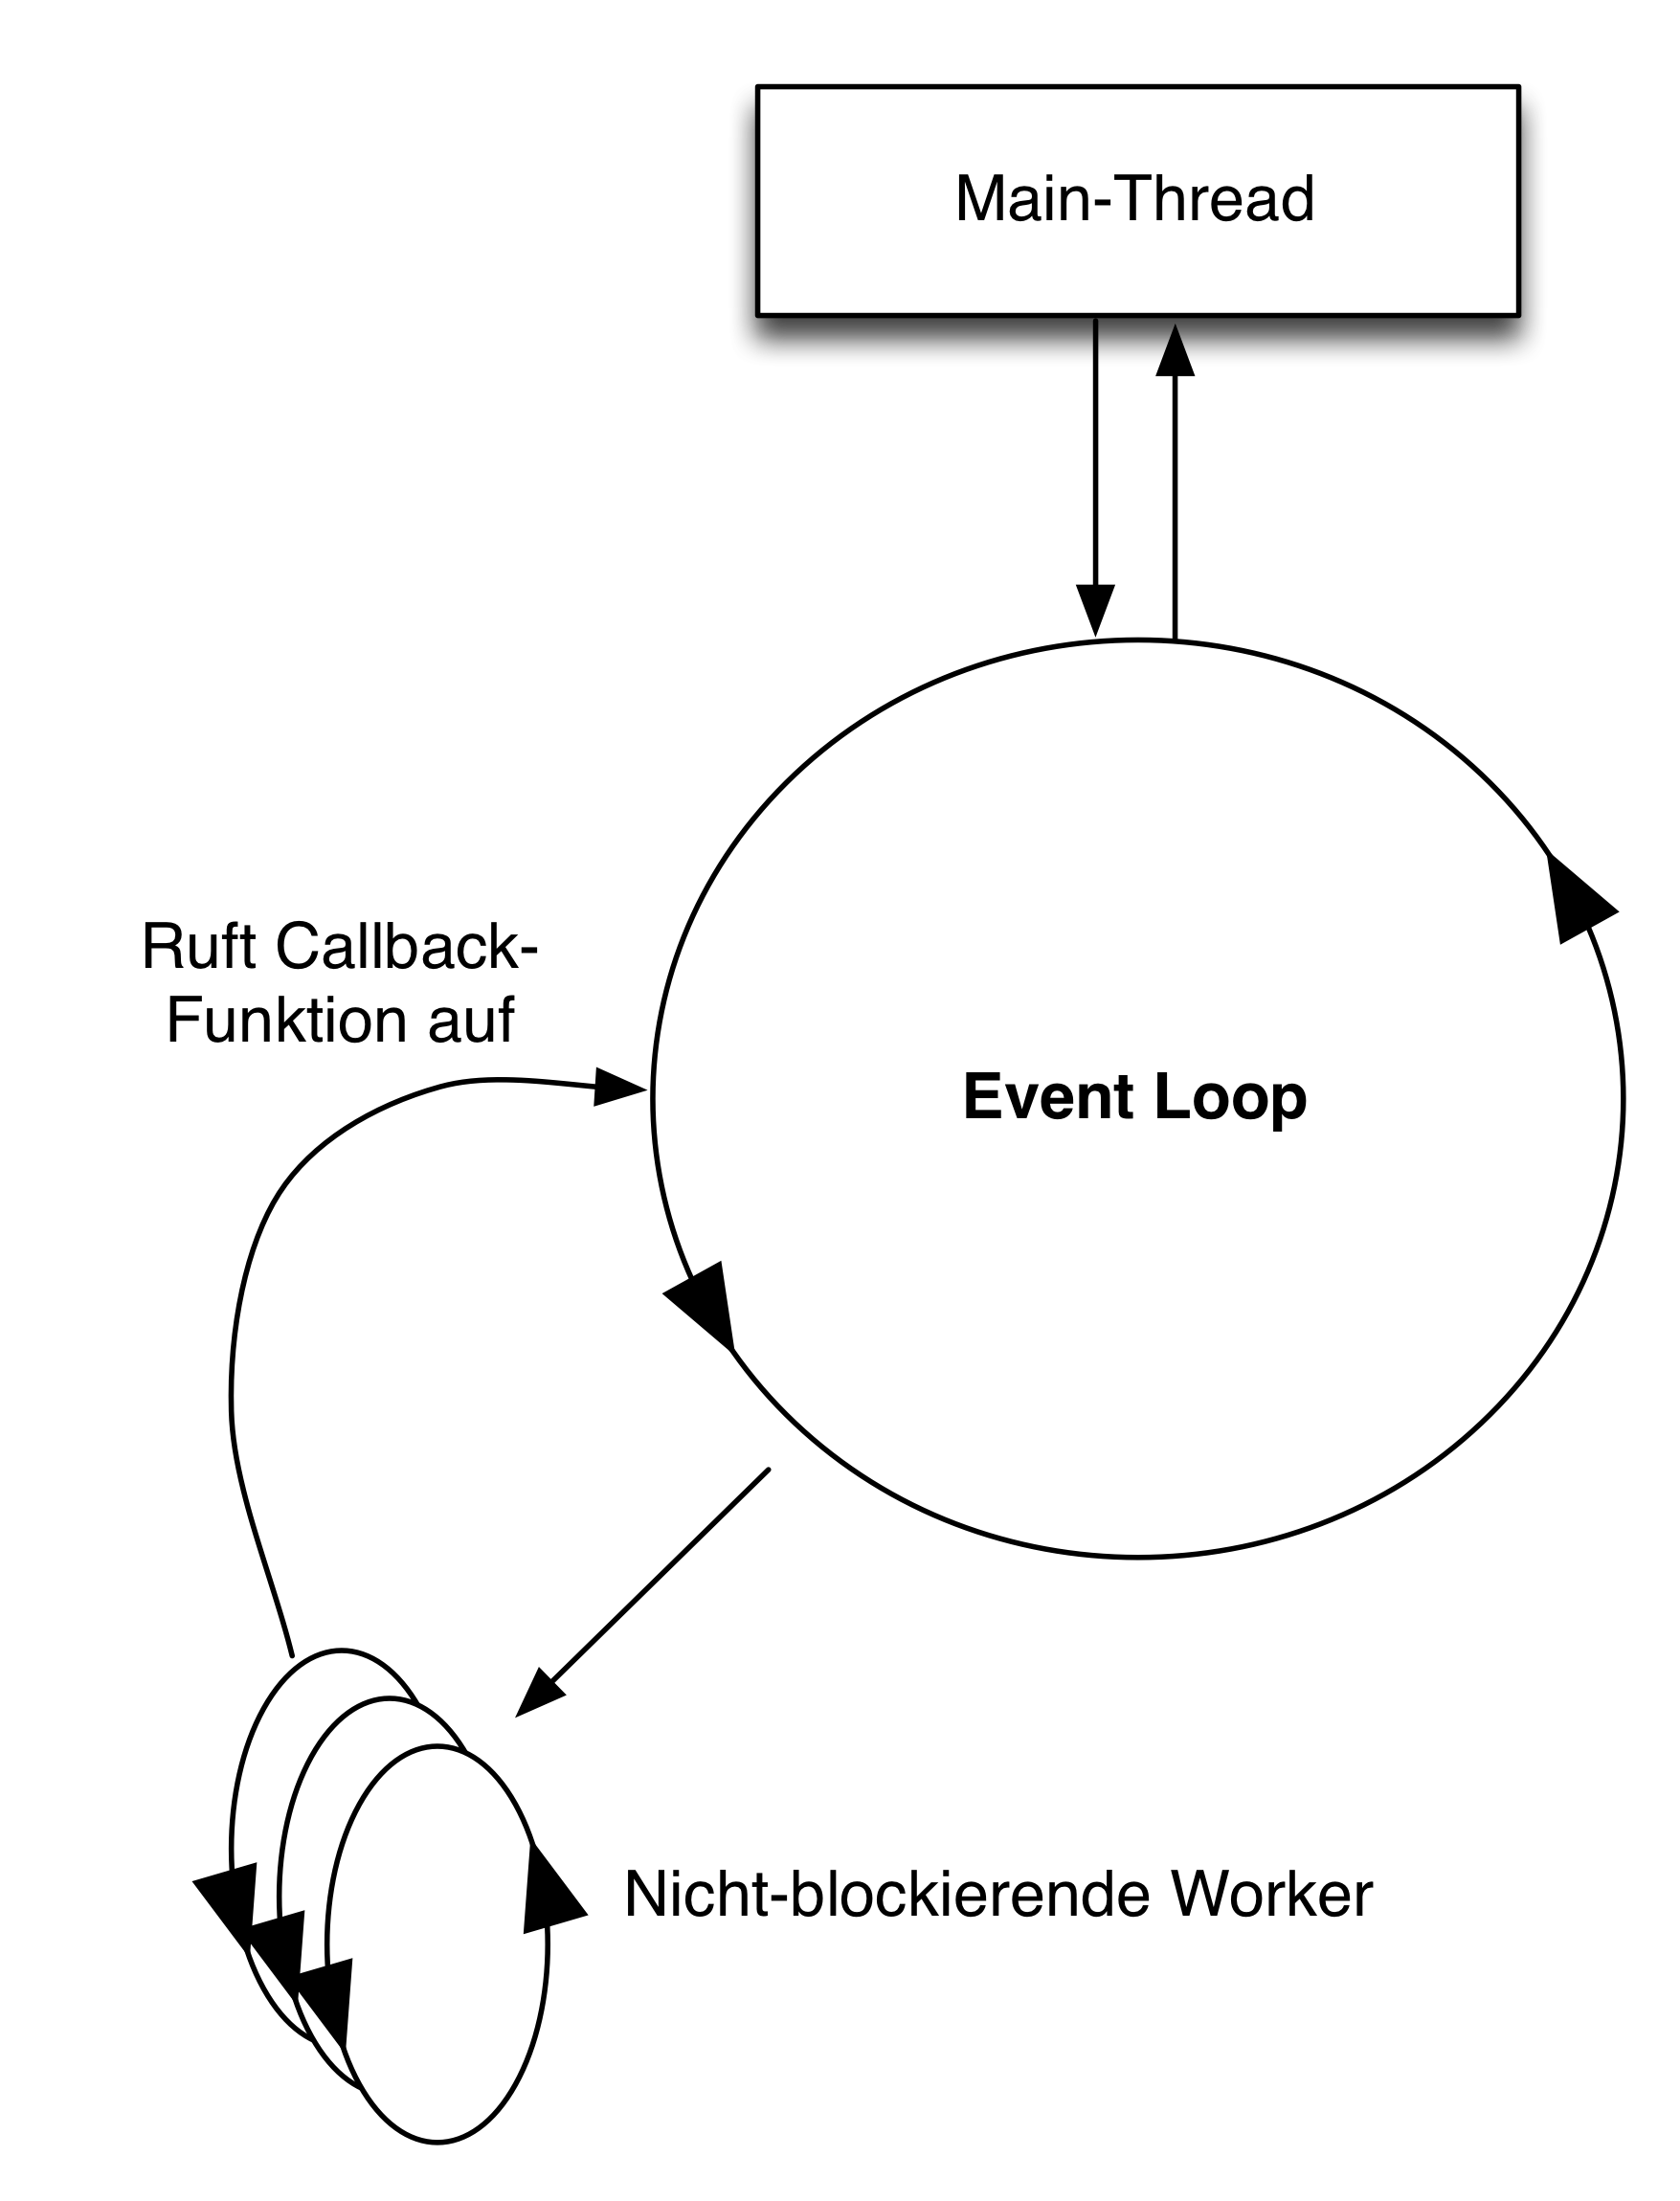
\includegraphics[width=0.4\textwidth]{images/nonblocking.png}
\caption[Event-Loop]{Event-Loop}
\label{fig:nonblocking}
\end{figure}

\subsection{\acl{CSP}}
\acf{CSP} ist eine von \textit{C.A.R. Hoare}, in einem Paper\footcite{CSP} erstmals vorgestellte formale Modellierung von nebenläufigen Prozessen und deren Kommunikation untereinander, mit Hilfe von Events und Nachrichten.

Hoare hat erkannt, dass in der Zukunft neue Algorithmen und Modelle benötigt werden, die horizontal skaliert werden können. Durch die zwingende Kommunikation zwischen den Prozessen ist ein spezifiziertes Konzept von Nöten, wodurch die Effizienz gesteigert werden kann. Die 1978 übliche Kommunikation über einen \textit{Shared Storage} und die Synchronisation über gegenseitigen Ausschluss, war zu komplex und zu fehleranfällig.\footcite[Introduction]{CSP}

Die in den folgenden Unterkapiteln verwendeten Symbole werden von Hoare in seinem Buch\footcite[Glossary of Symbols]{CSPBOOK} beschrieben.

\paragraph{Operatoren und Konstrukte in \acs{CSP}\footcite[Siehe][Kap. 1.1]{CSPBOOK}}
\ \\
Hoare definiert in seinem Buch zu \ac{CSP} einige Operatoren und Konstrukte, wovon die Essentiellen erläutert werden. Als Beispiel, wird das von Hoare in seinem Buch\footcite{CSPBOOK} verwendete Beispiel eines Schokoladenautomaten gezeigt, jedoch werden die Begriffe in die deutsche Sprache übersetzt.

\paragraph{Events}
\ \\
Events sind Aktionen, die jederzeit auftreten können. Dabei wird nicht zwischen eingehenden und ausgehenden Events unterschieden, diese Semantik ergibt sich durch den Kontext, der Verknüpfung der Prozesse. In Hoares Notation werden Events in Kleinbuchstaben geschrieben.
Im Beispiel eines einfachen Schokoladenautomaten existieren die folgenden zwei Events:

\begin{description}
\item[münze]\hfill \\
Das Einwerfen einer Münze in den Automaten.
\item[schokolade]\hfill \\
Das Entnehmen der Schokolade aus dem Auswurf des Automaten.
\end{description}

Um den Bezug zu \CA\ herzustellen, werden die Events um Channels erweitert, die Hoare in einem späteren Kapitel\footcite[Kap. 4.2]{CSPBOOK} im Buch definiert.
Wenn der Automat mit Channels definiert wird, besitzt dieser nun den Channel Münzeinwurf (\textit{in}) und den Channel Auswurf (\textit{out}).

Aus der Sicht des Automaten sehen die Events nun folgendermaßen aus:

\begin{description}
\item[in.münze]\hfill \\
Das Entnehmen einer Münze aus dem Münzeinwurf.
\item[out.schokolade]\hfill \\
Das Hineinlegen einer Schokolade in den Auswurf.
\end{description}

In nicht allen Fällen ist genau bekannt, um welches Event es sich auf dem Channel handelt. Damit eine Verbeitung dieser möglich ist, existieren die Operatoren \textit{?} und \textit{!}, mit denen Events in Variablen gespeichert werden (\textit{?}-Operator) oder Event aus Variablen auf einen Channel geschrieben werden können (\textit{!}-Operator). Da das Beispiel eines Schokoladenautomaten ungeeignet ist, wird ein neues Beispiel konstruiert. 

Hier handelt es sich um einen Automaten (\textit{COPY}), der aus einem Channel \textit{in} Events liest und den Wert in einen weiteren Channel \textit{out} schreibt. Dieser Automat hat die folgenden Events:

\begin{description}
\item[in?x]\hfill \\
Das Entnehmen eines Eventes aus dem \textit{in}-Channel und das Speichern in der Variable \textit{x}.
\item[out!x]\hfill \\
Das Hineinlegen des Wertes der Variable \textit{x} auf den \textit{out}-Channel.
\end{description}

Alle nachfolgenden Konstrukte werden mit Hilfe von Channels erklärt.

\paragraph{Prozesse}
\ \\
Ein Prozess wird durch eine Kombination aus verschiedenen Events, die sequentiell auftreten können definiert. In dem ersten Beispiel eines Schokoladenautomaten existiert der Prozess, der den  Schokoladenautomaten (\textit{SA}) definiert. Der Prozess \textit{SA} ist durch die Großbuchstaben als solches erkenntlich, wie es die Notation vorsieht. Auf ein Event muss stets ein Event oder ein Prozess folgen. Ein terminierbarer Automat kann dementsprechend nicht nach einem Event enden, sondern muss in einem anderen Prozess enden. Hierzu wird der Prozess \textit{STOP} definiert, der auf die eigentliche Ausführung des Prozesses folgt und den nicht mehr funktionsfähigen Schokoladenautomaten definiert.

\paragraph{Verkettung}
\ \\
Um die sequentielle Abfolge von Events, Prozessen und anderen Konstrukten darzustellen, definiert Hoare den 
$ \rightarrow $-Operator. Der Schokoladenautomat, der eine Münze annimmt, eine Schokolade auswirft und danach kaputt geht, sieht unter Verwendung des Operators wie folgt aus:
\[(\text{in.münze} \rightarrow (out.schokolade \rightarrow STOP))\]

Alternativ kann der Prozess auch benannt und die Klammern können entfernt werden, wodurch die Ausführung nun dementsprechend aussieht: 
\[SA = (\text{in.münze} \rightarrow \text{out.schokolade} \rightarrow STOP)\]

\paragraph{Rekursion}
\ \\
Einfache Verkettung ermöglicht bereits zu diesem Zeitpunkt die Modellierung von komplexen Prozessen. Allerdings existieren in Prozessen üblicherweise redundante Abläufe, die nicht modelliert werden können oder nicht vom Entwickler zur Modellierung vorgesehen sind. Um nicht den gesamten Ablauf einen Prozesses modellieren zu müssen, sieht die Notation Rekursion vor. Im Folgenden wird der nicht terminierende Automat \textit{SA} unter Anwendung der neuen Operatoren definiert:

\[SA = (\text{in.münze} \rightarrow \text{out.schokolade} \rightarrow SA)\]

Und das Beispiel des kopierenden Prozesses (\textit{COPY}) sieht folgendermaßen aus.

\[COPY = (\text{in?x} \rightarrow \text{out!x} \rightarrow COPY)\]

\paragraph{Parallelität}
\ \\
Die zu diesem Zeitpunkt vorgestellten Notation ermöglicht ausschließlich die gleichzeitige Ausführung eines Prozesses. Eine sequentielle Durchführung aller Prozesse ist zwar möglich, verkompliziert die einzelnen Prozesse, da ein Scheduling definiert werden muss. Gleichwohl sieht die Notation die parallele Ausführung mehrerer Prozesse vor. Bei der gleichzeitigen Ausführung von Prozessen werden Events, die in beiden Alphabeten vorkommen, synchron ausgeführt und Events, die nur in einem Prozess vorkommen vom anderen Prozess ignoriert. Durch die synchrone Ausführung von zwei gleichen Events ist es möglich die Kommunikation zwischen zwei Prozessen zu modellieren. Der Operator, der Prozesse parallel ausführt ist der \textit{||}-Operator. 

Zur Verdeutlichung werden die folgenden zwei Prozesse definiert:

\begin{addmargin}[1cm]{0cm}
$mensa:SA = \mu X \bullet (\text{in.münze} \rightarrow \text{out.schokolade} \rightarrow X)$\\\\
$student:KUNDE = \mu X \bullet (\text{geldzählen} \rightarrow \text{mensa.in.münze} \rightarrow \\ \text{mensa.out.schokolade} \rightarrow  X)$\\\\
$ (mensa:SA) || (student:KUNDE) $
\end{addmargin}

Der erste Prozess ist der bereits bekannte Schokoladenautomat. Hierbei handelt es sich um eine Instanz mit dem Namen \textit{mensa} und dem Prozesstyp \textit{SA}. $\mu X$ definiert eine Funktion mit dem Bezeichner \textit{X}, die dem Prozess \textit{SA} zugewiesen wird. Dadurch kann innerhalb der Funktion der Name \textit{X}, unabhängig vom Namen der Instanz,  verwendet werden. Der zweite Prozess ist ein Kunde mit dem Namen \textit{student}, der den Schokoladenautomat bedient. Er benutzt die Channels Münzeinwurf (\textit{in}) und Ausgabe (\textit{out}) des Schokoladenautomaten und zählt zu Beginn sein Geld. Damit beide Prozesse nun parallel auszuführen werden, wird der \textit{||}-Operator verwendet.

Die Aktion \textit{in.münze} des Mensa-Prozesses und die Aktion \textit{mensa.in.münze} des Studenten-Prozesses laufen simultan ab.\footcite[vgl][Seite 117]{CSPBOOK} Der Prozess blockiert, wenn der andere Prozess nicht bereit ist. Eine Art von Puffer der die Blockierung verhindern würde, müsste durch einen anderen Prozess modelliert werden.\footcite[vgl.][Seite 133]{CSPBOOK}.

\paragraph{Zusätzliche Konstrukte}
\ \\
Die oben vorgestellten Konstrukte reichen aus, um einen einfachen Automaten zu definieren, der immer den gleichen Ablauf hat. Für komplexere Algorithmen sind Verzweigungen von Nöten, um alternative Abläufe modellieren zu können. Die Notation sieht für diesen Fall den \textit{|}-Operator vor, der zwischen zwei Abläufen unterscheiden kann.

\subsubsection{Umsetzung der Konstrukte in core.async}
In \CA\ ist ein Prozess eine Sequenz von verschiedenen Befehlen, die entweder durch einen Thread ausgeführt oder in einem \textit{go}-Block in einen Zustandsautomat umgewandelt werden.

Die Kommunikation zwischen mehreren Prozessen erfolgt über Channels, die mit Hilfe der Funktion \textit{chan} erzeugt werden. Das Hineinlegen eines Wertes (Event), wird in der Notation nicht vom Herausnehmen unterschieden, außer das Event soll zwischengespeichert werden, in diesem Fall existieren die oben erklärten Operatoren (\textit{?} und \textit{!}). In \CA\ wird das Hineinlegen eines Werts in einen Channel mit den Funktionen \textit{>!!} (bei der Verwendung von Threads) oder \textit{>!} (in einem \textit{go}-Block) durchgeführt. Das Herausnehmen eines Werts aus dem Channel wird mit den Funktionen \textit{<!!} und \textit{<!} realisiert.

Alle übrigen Konstrukte, wie Rekursion, Verkettung, Verzweigungen etc. werden durch Clojure abgebildet.


\subsection{\acl{CPS} am Beispiel von JavaScript}
\label{sec:jscps}\acl{CPS} beschreibt einen Programmierstil, bei dem die Fortführung (Continuation) eines Programms an ein Unterprogramm übergeben wird. Zumeist werden die Continuations in Form von Funktionszeigern als Parameter an eine Funktion übergeben. In JavaScript werden diese als Callback-Funktionen bezeichnet. Der Einsatz von \acs{CPS} ermöglicht hier die asynchrone Abarbeitung von Funktionen. Betrachten wir das Code-Beispiel aus Listing \ref{lst:jscallback}. Im Folgenden werden die Bestandteile des Code Beispiels erklärt:
\begin{description}
\item[Die Funktion divides]\hfill \\
ermittelt, ob eine Zahl \textit{n} ein Teiler der Zahl \textit{m} ist und liefert einen boolschen Wert zurück.
\item[Die Funktion calcDividers]\hfill \\
nimmt eine Zahl \textit{n} entgegen sowie eine Continuation in Form einer Callback-Funktion. Mit Hilfe einer Schleife wird pro Iterationsschritt ein Teiler der Zahl \textit{n} ermittelt. Sind alle Teiler berechnet, so wird die übergebene Callback-Funktion aus der Parameterliste aufgerufen, als Parameter wird ein Array aller Teiler übergeben.
\item[Die Funktion printDividers] \hfill \\
repräsentiert die Continuation in dem Code-Beispiel. Das Programm wird an dieser Stelle fortgesetzt, sobald die Berechnung beendet ist. An dieser Stelle werden alle Teiler ausgegeben.
\item[Die Funktion main]\hfill \\
stellt den Entry-Point des Beispiels dar. Die Funktion \textit{calcDividers} wird für die Zahl \textit{65535} aufgerufen und \textit{printDividers} wird als Callback-Funktion übergeben.\\
\end{description}
\begin{lstlisting}[language=JavaScript,caption=JavaScript Callback Beispiel,label=lst:jscallback]
function divides(n, m) {
	return (m % n == 0);
}

function calcDividers(n, callback) {
	var dividers = Array();
	for(var i = 0; i<n; i++) {
		if(divides(i, n)) {
			dividers.push(i);
		}
	}
	callback(dividers);	
}

function printDividers(dividers) {
	var str = "{";
	for(var i=0; i<dividers.length; i++) {
		if(i > 0) {
			str = str.concat(", ");
		}
		str = str.concat(dividers[i]);
	}
	str = str.concat("}");
	console.log(str);
}

function main() {
	calcDividers(65535, printDividers);
	console.log("Calculation done.");
}

main();
\end{lstlisting}
\subsubsection*{Asynchronität}
Wird das Code-Beispiel auf Listing \ref{lst:jscallback} in einem JavaScript-Interpreter ausgeführt, so lässt sich kein asynchrones Verhalten der Anwendung, wie eingangs beschrieben, erkennen. Listing \ref{lst:jscallback_async} zeigt, wie \textit{calcDividers} asynchron aufgerufen werden kann. Hier wird die Funktion \mbox{\textit{calcDividers}} als Continuation mit Hilfe von \textit{setTimeout} an den JavaScript Event-Handler übergeben, der diese nach Ablauf des festgelegten Timeouts, in diesem Fall \textit{0 ms}, aufruft. Dieser Aufruf erlaubt, dass die nachfolgenden Befehle sofort ausgeführt werden. Wird das Code-Beispiel in einem JavaScript-Interpreter ausgeführt, so wird der Text ``Calculation started...'' vor der Ausgabe des Ergebnisses angezeigt. Das Ergebnis wird asynchron ausgegeben, wenn die Abarbeitung von \textit{calcDividers} abgeschlossen ist.
\begin{lstlisting}[language=JavaScript,caption=JavaScript setTimeout Beispiel,label=lst:jscallback_async]
...
function main() {
	setTimeout(function() { calcDividers(65535, printDividers) }, 0);
	console.log("Calculation started...")
}

main();
\end{lstlisting}

\subsection{Asynchrone Programmierung in Clojure}

Clojure ist eine Sprache, die zu Java- oder CIL-Bytecode und JavaScript (\acl{CLJS}) kompiliert werden und somit von einer \ac{JVM}, \ac{CLR} oder einem JavaScript-Interpreter ausgeführt werden kann.

In den beiden ersten Laufzeitumgebungen können Threads zur asynchronen und gleichzeitigen Verarbeitung von Befehlen verwendet werden. In JavaScript existiert der im vorherigen Kapitel vorgestellte Event-Handler.

Das folgende Beispiel, sowie alle restlichen Erläuterungen und Beispiele beziehen sich auf Clojure in Verwendung mit einer \ac{JVM}.

\subsubsection*{Beispiel anhand der Funktion \textit{future}}
Eine Methode eine Aufgabe auszulagern, die dann asynchron und concurrent abgearbeitet wird, funktioniert über die \textit{future}-Funktion (siehe Listing \ref{lst:clojure_future}). Die Funktion übergibt den übergebenen Body an einen Thread in einem \textit{ExecutionService} und gibt ein Future-Objekt an den Main-Thread zurück.

Der Main-Thread kann die Ausführung fortsetzen und weitere Aufgaben erledigen. Im Beispiel wird zusätzlich überprüft, ob es sich beim zurückgegebene Objekt um ein Future-Objekt handelt und mit der Funktion  \textit{realized?}, ob bereits ein Ergebnis vorliegt. Wenn die Aufgabe erledigt ist, kann der Main-Thread das Ergebnis der Berechnung über das Future anfragen, indem dieser mit der Funktion \textit{deref} oder dem Makro \textit{@} das Objekt dereferenziert. Falls die Aufgabe noch nicht erledigt ist, blockiert der Main-Thread solange, bis das Ergebnis vorliegt.

\begin{lstlisting}[language=Clojure,caption=Das asynchrone Ausführen von Befehlen mit der Funktion \textit{future},label=lst:clojure_future]
(println (-> (Thread/currentThread) (.getName)))
(let [f (future
          (Thread/sleep 1000)
          (println (-> (Thread/currentThread) (.getName)) "I am done")
          42)]
  (println (future? f))
  (println (realized? f))
  (Thread/sleep 2000)
  (println (realized? f))
  (println @f))
...
[stdout]:nREPL-worker-7
[stdout]:true
[stdout]:false
[stdout]:clojure-agent-send-off-pool-9 I am done
[stdout]:true
[stdout]:42
\end{lstlisting}

Dieses Beispiel verdeutlicht die Verwendung von Threads in Clojure. Falls eine gezieltere Kontrolle über die Definition und Ausführung von Threads gefordert ist, können über die \textit{Java-Interop}-Schnittstelle Threads selbstständig definiert oder es kann das \textit{ExecutionService}-Framework verwendet werden.

\subsubsection*{\acl{STM}}
Bei der gleichzeitigen Verarbeitung von Aufgaben und der Benutzung eines \textit{Shared Storages} existiert die Problematik, dass \textit{Race Conditions} entstehen können und die im Objekt gekapselten Daten somit inkonsistent werden können.

In Clojure garantiert das \acf{STM} bei der Veränderung von Referenzen, dass eine solche Inkonsistenz verhindert wird. Das \acs{STM} von Clojure verwendet hierfür ein \ac{MVCC} mit Snapshot Isolation. Dadurch kann das Phänomen des \textit{Write Skews}\footcite[S. Seite 17]{RENZSTATE} auftreten, das vom Entwickler erkannt und besonders behandelt werden muss.

Falls kein \ac{STM} erwünscht ist, kann auch das Synchronisationsprinzip von Java über Sperren verwendet werden, indem der kritische Abschnitt der Funktion \textit{locking} übergeben wird.

\subsection{Vergleich von \acs{CSP} und dem Actor Model}

Zur Modellierung von nebenläufigen Prozessen existieren neben \ac{CSP} auch andere Modelle. Ein verbreitetes Modell ist das Actor model (Aktorenmodell). Beide Modelle erfüllen den gleichen Zweck, dadurch haben sie viele Gemeinsamkeiten. Um \ac{CSP} besser verstehen zu können, ist eine Darstellung des Aktorenmodells und ein Vergleich beider Modelle von Vorteil.

Eine Gegenüberstellung von \ac{CPS}, Synchronisation mittels gegenseitigen Ausschlusses und \ac{CSP} macht nur bedingt Sinn, da es sich bei Ersterem um Programmierparadigmen handelt und bei \ac{CSP} um ein Designmuster.

Im Folgenden wird zuerst komprimiert das Aktorenmodell dargestellt und anschließend werden beide Modelle miteinander verglichen.

\subsubsection{Das Actor Model}
Das Aktorenmodell ist ein von \citeauthor{ACTORS} beschriebenes Modell zur Modellierung von künstlichen Intelligenzen, das sich für nebenläufige und parallele Programmierung eignet. Veröffentlicht wurde das Modell 1973 in dem Paper \textit{A Universal Modular ACTOR Formalism for Artificial Intelligence}\footcite{ACTORS}. Von \citeauthor{ACTORSNEW} wurde das Modell mit dem Paper \textit{Actor Model of Computation: Scalable Robust Information Systems}\footcite{ACTORSNEW} 2011 aufbereitet. 

Aktoren bestehen aus folgenden fundamentalen Teilen:

\begin{description}
\item[Prozess]\hfill \\
Ein Aktor benötigt einen Prozess, der die Aufgaben des Aktors ausführt. Üblicherweise ist das ein Thread.
\item[Speicher]\hfill \\
Zustände des Aktors werden in einem Speicher gesichert, damit unterschiedlich auf Nachrichten reagiert werden kann.
\item[Kommunikation] \hfill \\
Aktoren müssen untereinander kommunizieren können und sich Nachrichten senden können.
\end{description}

Ein Aktor ist für sich alleine genommen kein Aktor, erst in einem Aktorensystem existiert er. Das Aktorensystem stellt ein Kommunikationsmedium bereit, das nach \glqq best effort\grqq\ versucht die Nachrichten zu übertragen. Dementsprechend können Nachrichten verloren gehen oder andere Nachrichten überholen. Aktoren verfügen über eine Adresse, worüber andere Aktoren ihnen Nachrichten senden können. Nachrichten werden in das Aktorsystem gelegt und ein Aktor bekommt \glqq irgendwie\grqq\ die Nachricht zugestellt, wenn er sie benötigt. Puffer, Mailboxen und Queues werden im Aktorenmodell \textbf{nicht} explizit definiert\footcite[Seite 3, Rechte Spalte]{ACTORSNEW}. Die technische Umsetzung übernehmen die Implementierungen. Ein Aktor verarbeitet mit seinem Prozess nur eine Nachricht zu einem Zeitpunkt und da Aktoren keinen gemeinsamen Speicher benutzen dürfen, können auch keine Race-Conditions auftreten. Das Aktorenmodell ist nicht deterministisch, da die Kommunikation zwischen Aktoren nicht genau definiert ist und die Nachrichten zufällig beim Empfänger eintreffen können, wodurch Determinismus nicht garantiert werden kann.

\subsubsection{Unterschiede und Gemeinsamkeiten}
Es sind beides theoretische Modelle zur Beschreibung von Parallelität und Nebenläufigkeit. 
Beide Modelle unterscheiden sich bereits in ihrer Art der Definition. \ac{CSP} ist eine Prozess-Algebra und basiert auf mathematischen Gesetzen, wodurch keine Unklarheiten existieren. Das Aktorenmodell hingegen orientiert sich an der Physik und kann aufgrund dessen bestimmte Bereiche nicht genau spezifizieren, sodass Axiome als Begründung verwendet werden, wodurch das Modell vereinfacht wird. Das Aktorenmodell ist aufgrund der Axiome nicht deterministisch. Determinismus muss zusätzlich spezifiziert werden. Abläufe in \ac{CSP} sind deterministisch. Um die Automaten simpel zu halten, kann Nichtdeterminismus mit einem besonderen Operator ($\sqcap$) speziell modelliert werden.\\
Das Aktorenmodell definiert nicht, wie eine Nachricht empfangen wird. Dies kann über einen blockierenden Aufruf passieren oder eine eingehende Nachricht kann eine Methode aufrufen, wie es zum Beispiel in dem Aktorenframework \textit{Akka} umgesetzt wird. In \ac{CSP} kann es nur blockierende bzw. parkende Operationen geben, da ein Prozess auf mehrere Channels gleichzeitig warten kann.\\
Der Datenaustausch zwischen zwei Prozessen in \ac{CSP} ist simultan, sodass ein Prozess blockiert, wenn kein anderer Prozess mit der gegensätzlichen Aktion auf den Channel zugreift. Ein Puffer muss mit einem weiteren Prozess modelliert werden. Die Kommunikation mit Nachrichten zwischen zwei Aktoren passiert asynchron, da das Aktorensystem die Zustellung der Nachrichten übernimmt. Eine mengenmäßige Begrenzung ist nicht vorgesehen. In technischen Implementierungen des Aktorenmodells wie \textit{Akka} existieren Begrenzungen seitens der Konfiguration oder der Hardware. Zudem sichert \textit{Akka} auch zu, dass Nachrichten nicht verloren gehen und sich nicht überholen können.

\section{Die Bibliothek core.async}

\subsection{\acs{API} Code-Beispiele}
Dieses Kapitel demonstriert die Basis-Funktionalität des Frameworks anhand von Code-Beispielen. Zwecks Vereinfachung der Beispiele wird eingangs die Funktion \textit{read-chan} aus Listing \ref{lst:readchan}\  definiert, die eine einheitliche Ausgabe der Werte auf dem ihr übergebenen Channel realisiert. Diese Funktion entnimmt mit \textit{loop} und \textit{recur} solange alle Werte aus einem Channel, bis dieser geschlossen wird. Das ein Channel geschlossen ist, wird durch das Entnehmen des Wertes \textit{nil} festgestellt.
\begin{lstlisting}[language=Clojure,caption=\textit{read-chan} Hilfsfunktion,label=lst:readchan]
(defn read-chan
  ([c] (read-chan "" c))
  ([str c]
  (thread
    (loop [val (<!! c)]
      (when (not= val nil)
        (println str val)
        (recur (<!! c))))
      (println "END."))))
\end{lstlisting}
\subsubsection{\textit{Go}-Blocks}
Das folgende Code Beispiel aus Listing \ref{lst:goblock}\ demonstriert den Parking-Mechanismus. Zu Beginn wird  ein ungepufferter Channel \textit{c} erzeugt. Anschließend wird mittels \textit{>!} und \textit{<!} in Kombination mit \textit{go} darauf zugegriffen. Ist der Channel belegt, so wird die \textit{>!} Funktion geparkt. Ein ähnliches Verhalten ist bei \textit{<!} erkennbar, welche geparkt wird, wenn kein Wert auf dem Channel vorliegt. Ist ein Wert vorhanden, so wird dieser vom Channel entfernt und auf der Konsole ausgegeben.
\begin{lstlisting}[language=Clojure,caption=\textit{Go}-Blocks,label=lst:goblock]
(let [c (chan)]
  (go
    (>! c "test"))
  (go
    (println (<! c))))
\end{lstlisting}
\subsubsection{Threads}
Das obige Beispiel aus Listing \ref{lst:goblock}\ lässt sich auch mit blockierenden Funktionen in Threads ausführen. Die Korrelate zu den Put- und Take-Operation sind hier \textit{>!!} und \textit{<!!}, welche den jeweiligen Thread, in dem sie ausgeführt werden beim Lesen bzw. Schreiben blockieren (siehe Listing \ref{lst:thread}).
\begin{lstlisting}[language=Clojure,caption=Thread,label=lst:thread]
(let [c (chan)]
  (thread
    (>!! c "test"))
  (thread
    (println (<!! c))))
\end{lstlisting}
\subsubsection{Timeout}
Channels werden in ihrer Lebensdauer zeitlich beschränkt, wenn ihre Erzeugung mit Hilfe der \textit{timeout}-Funktion erfolgt ist. Diese Kanäle werden nach Ablauf des Timeouts automatisch geschlossen. Das Beispiel aus Listing \ref{lst:timeout} demonstriert dieses Verhalten.\\
\\
Zu Beginn wird ein Channel mittels \textit{timeout} erzeugt und neuer Wert asynchron mit Hilfe von \textit{put!} darauf abgelegt. In einem Thread werden nun, wie in der Funktion \textit{read-chan} aus Listing \ref{lst:readchan}\ solange Werte vom Channel abgerufen, bis dieser seine Schließung nach vier Sekunden mittels \textit{nil}-Wert signalisiert.
\begin{lstlisting}[language=Clojure,caption=Timeout,label=lst:timeout]
(let [c (timeout 4000)]
  (put! c "test")
  (thread
  (loop [val (<!! c)]
    (when (not= val nil)
      (println val)
      (recur (<!! c))))
    (println "timeout")))
\end{lstlisting}
\subsubsection{Filter}
Channels können mit einem Filter versehen werden, der die eingehenden Werte auf die Erfüllung eines Prädikats prüft. Das Beispiel aus Listing \ref{lst:filter} veranschaulicht die Verwendung der \textit{filter>} Funktion, die diese Funktionalität bereitstellt. Die Funktion erhält ein Prädikat, sowie einen Ausgabe-Channel und gibt einen Eingabe-Channel zurück. Der von der Funktion \textit{filter>} erzeugte Prozess prüft, ob die eingehenden Werte vom Typ String sind. Werte, die dem Prädikat entsprechen, werden auf den Ausgabe-Channel gelegt, alle anderen werden verworfen.

\begin{lstlisting}[language=Clojure,caption=Filter,label=lst:filter]
(let [out (chan)
      c (filter> string? out)]
  (thread
    (>!! c "abc")
    (>!! c 123))
  (read-chan out))
\end{lstlisting}
\subsubsection{Buffer}
Channels sind standardmäßig ungepuffert, d.h. es kann maximal ein Wert abgelegt werden. Die Schreiber werden solange geparkt bzw. blockiert, bis der Channel wieder frei ist. Dieses Verhalten kann bei der Erzeugung des Channels eingestellt werden (siehe Listing \ref{lst:buffer}). Im Listing wird bei der Erzeugung des Channels ein Puffer der Größe vier übergeben, der zuvor mit der Funktion \textit{buffer} erzeugt wurde. Alternativ kann die Größe des Kanal-Puffers direkt der \textit{chan}-Funktion als Zahlwert übergeben werden. Der Channel akzeptiert nun vier Werte, anschließend werden alle Schreiber geparkt bzw. blockiert.
\begin{lstlisting}[language=Clojure,caption=Buffer,label=lst:buffer]
(let [c (chan (buffer 4))]
  (dotimes[n 4]
    (>!! c n))
  (dotimes[n 4]
    (println (<!! c))))
\end{lstlisting}

\subsection{ClojureScript}
ClojureScript ist ein Compiler, der eine Kompilierung von Clojure Code zu JavaScript ermöglicht.\footcite{CLJS} Das core.async Framework ist ClojureScript kompatibel, dennoch werden vereinzelte vorgestellte Konstrukte nicht unterstützt. Da JavaScript single-threaded ist, existiert keine Thread-Unterstützung, demnach stehen die Funktionen \textit{>!!}, \textit{<!!}, \textit{thread}, sowie alle weiteren auf Threads basierenden Funktionen (alle mit der Endung \textit{!!}) nicht zur Verfügung.

\subsection{Beispiele von Hoare zu \acs{CSP}}
Tony Hoare hat in seinem Paper\footcite{CSP} diverse Beispiele erläutert, in denen \ac{CSP} angewendet wird. Einige der einfacheren Beispiele sind in \textit{core.async} implementiert worden und sind auf Github\footnote{\url{https://github.com/serofax/CSPHoareExamplesCoreAsync}} zu finden.

Hoare teilt seine Beispiele in vier Bereiche. 

\begin{description}
\item[Coroutines]\hfill \\
Koroutinen sind Prozesse, die Daten von einem oder mehreren Channels entgegennehmen und diese dann in meistens veränderter Form ausgeben.

In \CA\ sind alle Koroutinen umgesetzt worden und befinden sich in der Datei \textit{coroutines.clj}.
\item[Subroutines and Data Representation]\hfill \\
Subroutinen sind Prozesse, die aus Koroutinen zusammengesetzt sind und eine bestimmte Aufgabe erfüllen, wie z. B. das rekursives Berechnen der Fakultät.

Sechs Beispiele definiert Hoare in seinem Paper. In \CA\ umgesetzt wurden lediglich die rekursive Berechnung der Fakultät und einen Divisionsprozess, der aus einem Dividenden und einem Divisor den Quotienten und den Rest errechnet. Diese beiden Beispiele sind in der Datei \textit{subroutines.clj} zu finden.
\item[Monitores and Scheduling] \hfill \\
In diesen Beispielen werden Prozesse definiert, die die Aufgabe eines Monitors übernehmen, um den gleichzeitigen Zugriff auf eine oder mehrere Ressourcen zu koordinieren.

Von den Monitorbeispielen sind der Integer-Monitor und das Beispiel der Dining Philosopers umgesetzt worden. Die Monitore in diesem Beispiel sind die Gabeln und der Raum. Die Integer-Monitore ist in der Datei \textit{semaphore.clj} zu finden und das Philosophen-Beispiel in der Datei \textit{philosophers.clj}.
\item[Miscellaneous] \hfill \\
Die Beispiele dieses Kapitel ließen sich in keine der oberen drei Kapitel einteilen. Von diesen wurde keines in \CA\ umgesetzt.
\end{description}

\section{Zusammenfassung und Fazit}

Zu Beginn wurde erklärt, was asynchrone Programmierung bedeutet und weshalb ein nicht blockierendes \acs{I/O}-Modell hierzu benötigt wird. Diese beiden Begriffe wurden mittels JavaScript- und Clojure-Code anschaulich dargestellt. Zudem wurde das Programmierparadigma \acf{CPS}, das häufig in JavaScript zum Einsatz kommt, erläutert.\\
Zur Einführung in die Design Prinzipien von \textit{core.async} wurde das Channel- und Prozess-Prinzip aus Tony Hoare's Prozess-Algebra \acf{CSP} zur Modellierung nebenläufiger Prozesse erklärt. Es wurde gezeigt, dass \acs{CSP} eine sinnvolle Methode ist, um effizient, unter Ausschluss von  Race-Conditions, nebenläufige Modelle zu konstruieren, die von modernen Multi-Core-Prozessoren parallel ausgeführt werden können.\\
Zur Darstellung der Vor- und Nachteile von \acs{CSP}, wurde ein Vergleich zwischen diesem und dem Aktorenmodell angestellt. Das Aktorenmodell ist wie \acs{CSP} ein Prinzip zur Modellierung von Nebenläufigkeit. Es wurde festgestellt, dass keines der Modelle gegenüber dem Anderen präferiert werden kann. Der Entwickler muss nach den bestehenden Anforderungen entscheiden, welches Modell den fachlichen Anforderungen besser entspricht, so auch beim Einsatz von \textit{core.async}. Jedoch sollten auch die Unterschiede der Implementierungen in Betracht gezogen werden, die eventuelle Nachteile des theoretischen Modells aufwiegen.\\
Das darauffolgende Kapitel dieser Ausarbeitung, befasste sich mit der Darstellung der Basis-Funktionalität der \acs{API} von \textit{core.async}, die mit Code-Beispielen demonstriert wurde. Die Bibliothek wirkt sehr stabil. Der Umfang der \acs{API} ist für eine Version im Alpha-Stadium beachtlich und kann bereits jetzt produktiv in kleineren Projekten eingesetzt werden. Es ist hervorzuheben, dass - ausgenommen Thread-basierter Konstrukte - \textit{core.async} kompatibel zu ClojureScript ist und der Clojure-Code demnach zu JavaScript kompiliert werden kann. Dies erleichtert die Modellierung von Quasi-Parallelen (single threaded) Prozessen in JavaScript erheblich und schafft neue Möglichkeiten.\\
Dieses Projekt hat uns tiefe Einblicke in diverse hochinteressante Programmierparadigmen zur Modellierung von Nebenläufigkeit und Parallelität gewährt und uns persönlich weiter gebracht.










\pagenumbering{Roman}
\setcounter{page}{\value{last_roman}}
\chapter*{Abkürzungsverzeichnis}
\addcontentsline{toc}{chapter}{Abkürzungsverzeichnis}
\markboth{Abkürzungsverzeichnis}{Abkürzungsverzeichnis}
\begin{acronym}
%
%ALPHABETISCH SORTIEREN!!!
%
\acro{API}{Application Programming Interface}
\acro{CLJS}{ClojureScript}
\acro{CLR}{Common Language Runtime}
\acro{CPS}{Continuation Passing Style}
\acro{CSP}{Communicating Sequential Processes}
\acro{I/O}{Input/Output}
\acro{JVM}{Java Virtual Machine}
\acro{MVCC}{Multiversion Concurrency Control}
\acro{STM}{Software Transactional Memory}
\end{acronym}
\listoffigures
%\phantomsection
\addcontentsline{toc}{chapter}{Tabellenverzeichnis}
\listoftables

\renewcommand{\lstlistlistingname}{Listingverzeichnis}
\lstlistoflistings
\nocite{*}
\printbibliography[heading=bibintoc,title={Literaturverzeichnis}]




%\chapter{Einleitung}
Diese Ausarbeitung befasst sich mit \CA , einer Bibliothek zur asynchronen Programmierung in der Programmiersprache Clojure. Es werden zunächst die grundlegenden Begrifflichkeiten erklärt, andere State-of-the-Art Programmierparadigmen, Entwurfsmuster und Frameworks betrachtet und anschließend mit \CA\ verglichen. Anhand von Beispielen aus dem \acf{API} des Frameworks, wird der aktuelle Entwicklungsstand des noch im Alpha-Stadium befindlichen Frameworks gezeigt und dessen Potential bewertet.
\comment{Bewerten? Wenn API-Beispiele gelesen nochmals validieren.}
\acresetall
%\chapter{Grundlagen}

%Section Was bedeutet asynchrone Programmierung?
\section{Was bedeutet asynchrone Programmierung?}
Zu Beginn stellt sich die Frage nach der Erläuterung des Begriffs \textit{asynchrone Programmierung}. Betrachten wir eine imperative Programmiersprache ohne Multithreading, so lässt sich dieser Begriff leicht erklären. Eine Anwendung in einem imperativen Kontext hat ihren Entry-Point in der ersten Zeile des Programmcodes. Der Code wird streng sequentiell abgearbeitet. Jeder Befehl blockiert die Anwendung, solange bis seine Abarbeitung beendet ist. Dieses Verhalten einer Anwendung wird als \textit{synchrone} Abarbeitung einer Befehlsfolge bezeichnet. Der Nachteil ist hier, dass Wartezeiten zwischen Berechnungen entstehen. Lange Berechnungen reduzieren die Performanz der Anwendung, da stets auf ihre Beendigung gewartet werden muss. Hier kommt \textit{asynchrone Programmierung} zum Tragen. Der Begriff beschreibt eine sequentielle Befehlsabarbeitung, bei der keine Wartezeit zwischen Berechnungen entsteht. Grundlage hierfür stellen ein nichtblockierendes I/O-Modell, welches im nächsten Kapitel erklärt wird, sowie diverse Programmierparadigmen dar.



%Section Blockierende nich blockierende IO
\section{Blockierende und nichtblockierende \acs{I/O}}
 \label{sec:nonblocking}Ein nichtblockierendes I/O-Modell ermöglicht die Verarbeitung von Befehlen bei zeitintensiven Berechnungen oder Datenbankabfragen ohne dass der Main-Thread der Anwendung blockiert wird. Es muss nicht auf das Ergebnis der Berechnung gewartet werden, bevor der nächste Befehl ausgeführt werden kann. Der Mechanismus kann beispielsweise mit Hilfe einer Event-Loop umgesetzt werden, die Vorgänge in sogenannten Worker-Threads auslagert und diesen jeweils eine Callback-Funktion übergibt. Die Funktion wird im Main-Thread aufgerufen, sobald der jeweilige Berechnungsvorgang beendet ist (siehe Abb. \ref{fig:nonblocking}). Diese Technik nennt sich \acf{CPS} und wird im Kapitel \ref{sec:jscps} am Beispiel von JavaScript erklärt. Ein nichtblockierendes I/O-Modell stellt die Grundlage für asynchrone Programmierung dar.
\begin{figure}[H]
\centering
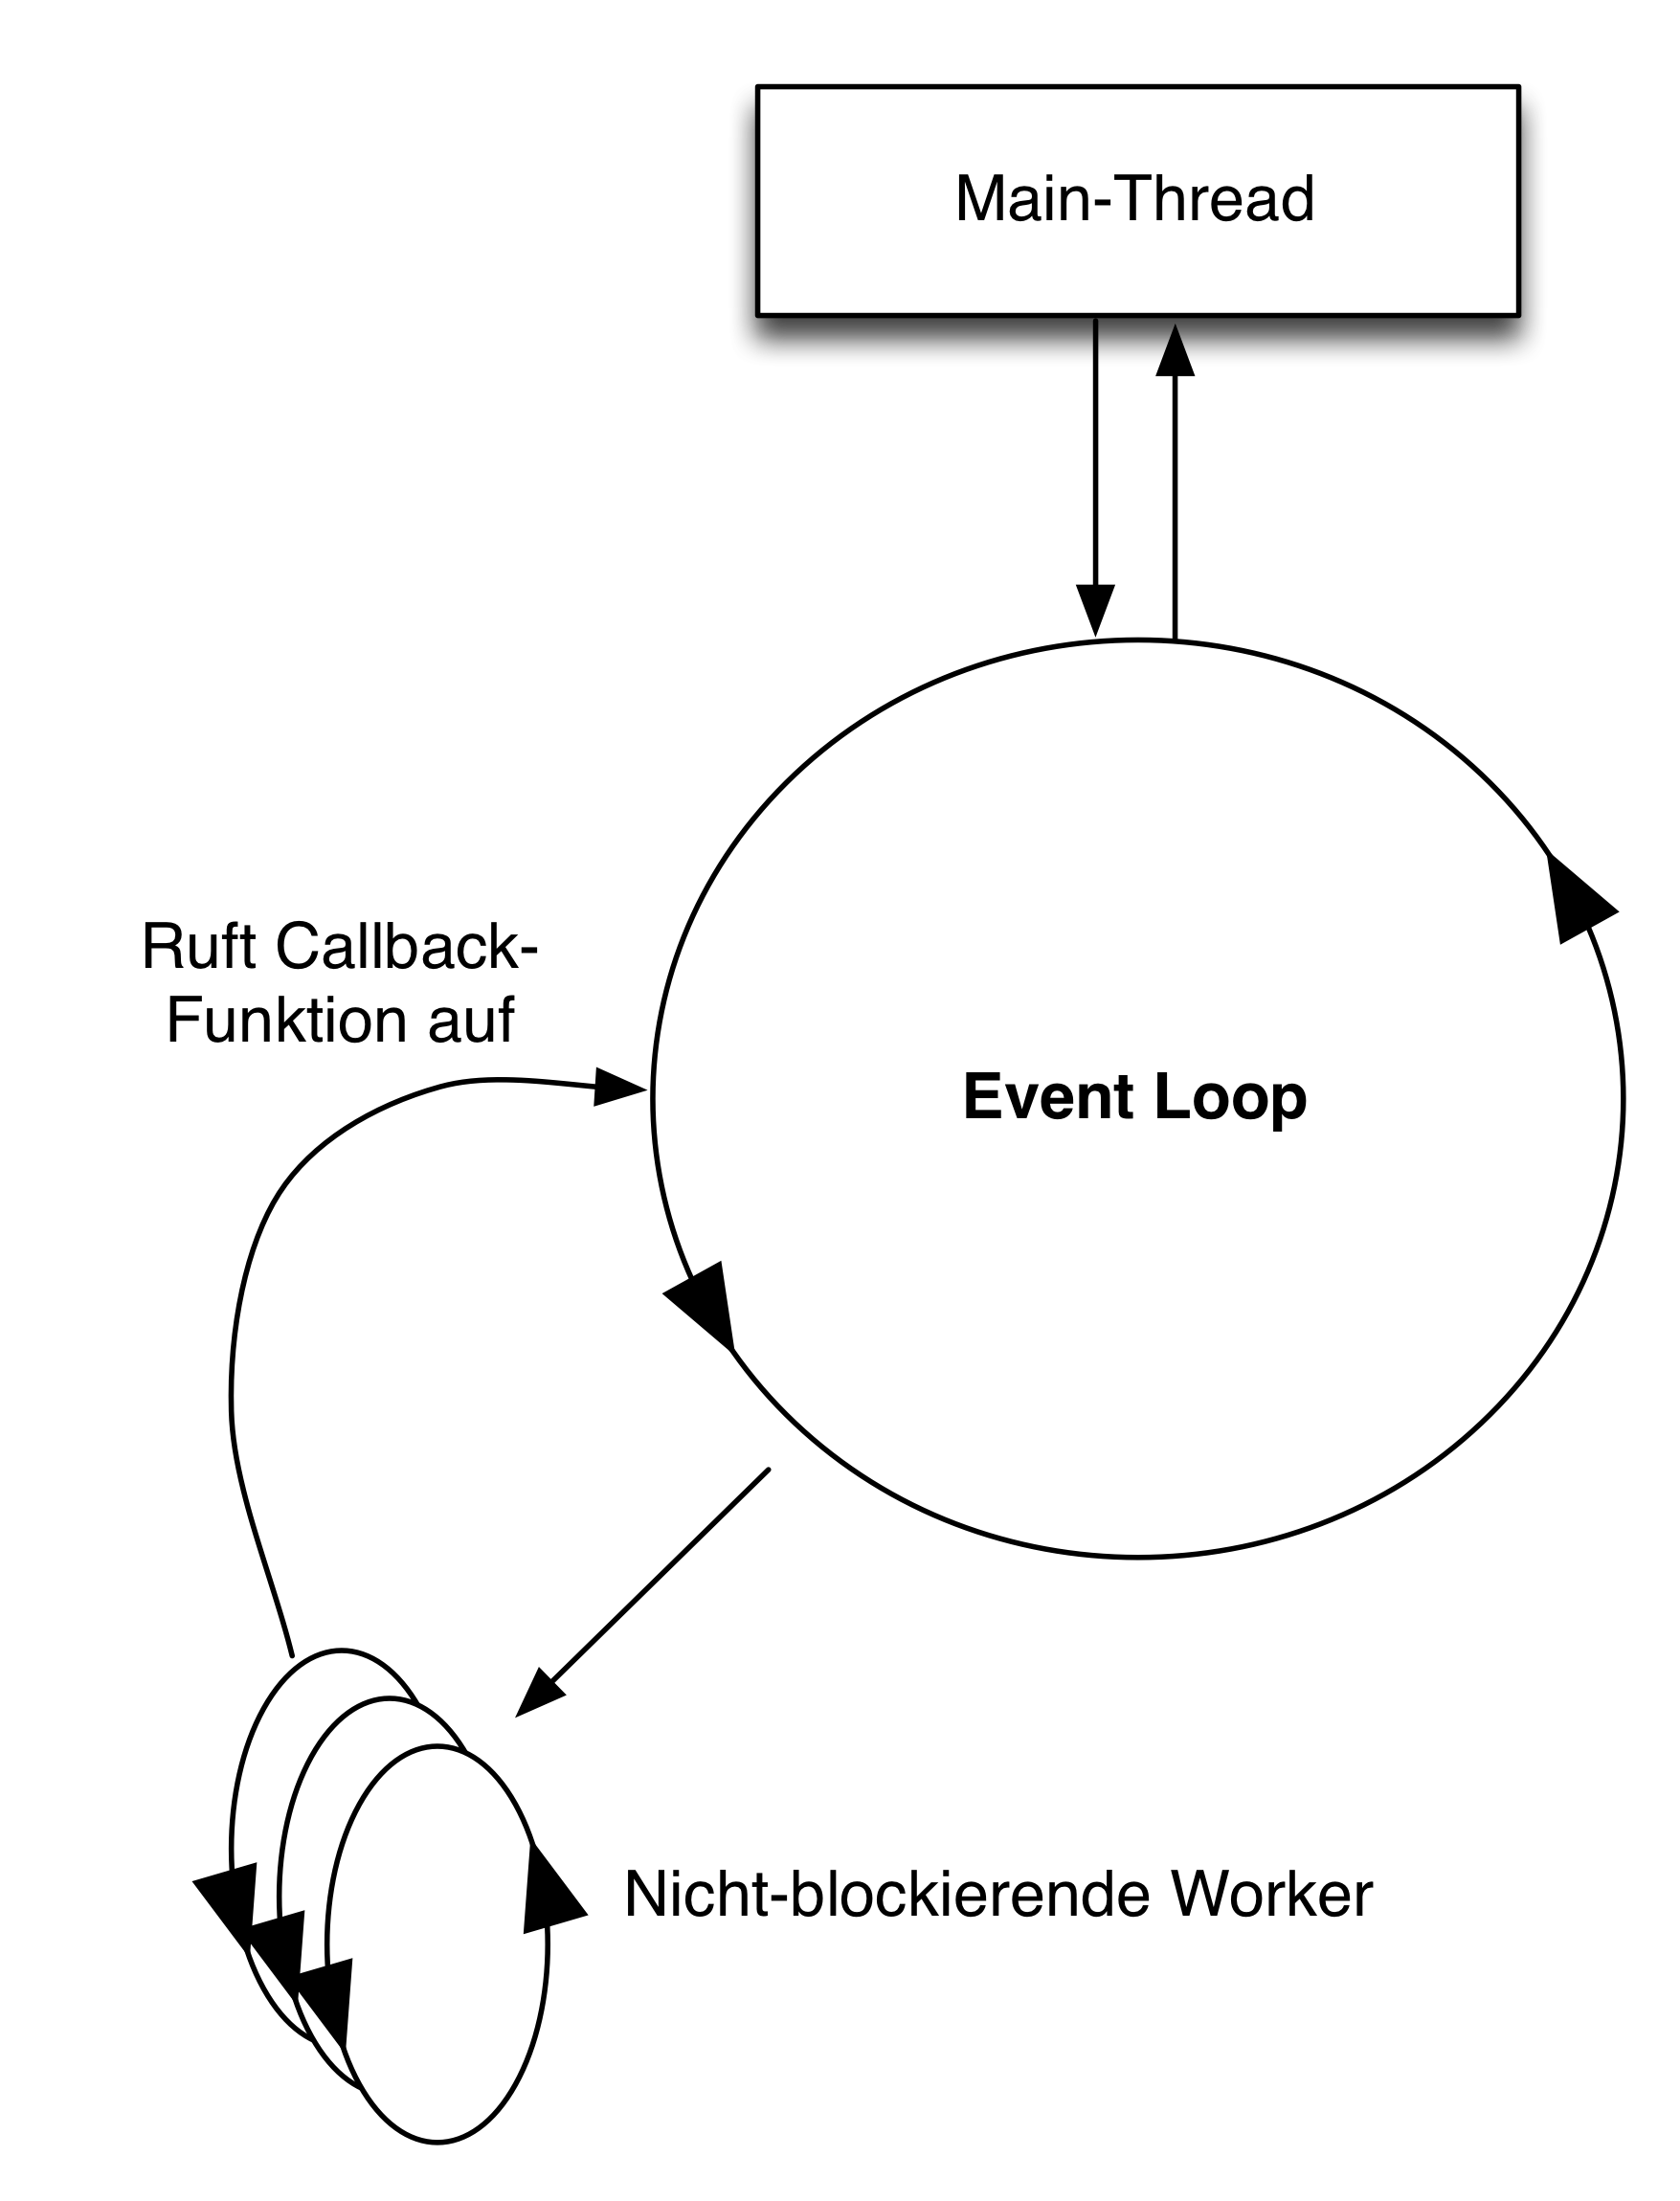
\includegraphics[width=0.4\textwidth]{images/nonblocking.png}
\caption[Event-Loop]{Event-Loop}
\label{fig:nonblocking}
\end{figure}
\acresetall


%Section CSP
\section{\acl{CSP}}
\acf{CSP} ist eine von \textit{C.A.R. Hoare} in seinem Paper\footcite{CSP} \textit{Communication Sequential Processes} 1978 erstmals vorgestellte formale Beschreibung von gleichzeitigen Prozessen und deren Kommunikation untereinander mit Events und Nachrichten.

Als Begründung, warum er ein solches System definiert hat, gibt Hoare an, dass in Zukunft neue Algorithmen benötigt werden, die parallel ausgeführt werden. Durch die zwingende Kommunikation unter den Prozessen ist ein neues Konzept von Nöten, dass das genau spezifiziert und somit die  Effizient steigert. Die damalige Synchronisation über \textit{shared Storage} hat ihm nicht gefallen, da sie zu fehleranfällig und zu komplex war.\footcite[Introduction]{CSP}

Die verwendeten Symbole werden von \textit{C.A.R. Hoare} in seinem Buch\footcite[Glossary of Symbols]{CSPBOOK} beschrieben und können da nachgeschlagen werden.
\subsection[Operatoren und Konstrukte in \acs{CSP}]{Operatoren und Konstrukte in \acs{CSP}\footcite[Siehe][Kap. 1.1]{CSPBOOK}}

Hoare definiert sehr viele Operatoren und Konstrukte. Die Essentiellen von ihren werden nun erläutert. Für Beispiele, wird das von Hoare gerne in seinem Buch\footcite{CSPBOOK} verwendete Beispiel eines Schokoladenautomaten verwendet, jedoch wurden die Begriffe ins Deutsche übersetzt.

\subsubsection{Events}
Events sind Aktionen, die auftreten können. Zwischen eingehenden und ausgehenden Events wird nicht unterschieden. In Hoares Notation werden Events in Kleinbuchstaben geschrieben.
Zum Beispiel bei einem einfachen Schokoladenautomaten gäbe es folgende Events:

\begin{addmargin}[1cm]{0cm}
münze - Das Einwerfen einer Münze in den Automaten.\\
schokolade - Das Entnehmen der Schokolade aus dem Auswurf des Automaten.
\end{addmargin}

Um den Bezug zu \CA\ herzustellen, erweitern wir die Events um Channels, womit sich Hoare erst in einem späteren Kapitel\footcite[Kap. 4.2]{CSPBOOK} im Buch befasst. Stellen wir uns nun den Münzeinwurf (\textit{in}) und den Auswurf (\textit{out}) des Automaten als Channel vor. Die Events aus Sicht des Prozesses sehen nun wie folgt aus:

\begin{addmargin}[1cm]{0cm}
in.münze - Das Entnehmen einer Münze aus dem Münzeinwurf.\\
out.schokolade - Das Hineinlegen einer Schokolade in den Auswurf.
\end{addmargin}

Um Variablen ins Spiel zu bringen gibt es den ?-Operator und den !-Operator. Da das Beispiel dafür ungeeignet ist, wird ein Neues definiert. Nun gibt es einen Automaten (\textit{COPY}), der aus seinem in-Channel liest und den Wert in seinen out-Channel schreibt. Folgende Events gäbe es:

\begin{addmargin}[1cm]{0cm}
in?x - Das Entnehmen von Irgendwas aus dem in-channel und das Speichern in der Variable x.\\
out!x - Das Hineinlegen von dem Wert in der Variable x auf den out-channel.
\end{addmargin}

Alle weiteren Konstrukte werden anhand von Channels erklärt.

\subsubsection{Prozesse}
Ein Prozess definiert sich durch eine Kombination aus verschiedenen Events, die sequentiell hintereinander ausgeführt werden. In unserem ersten Beispiel existiert nur ein Prozess und zwar der Schokoladenautomat \textit{SA}, der durch die Großbuchstaben auch als solches erkenntlich ist. Um einen Automaten terminierbar darzustellen kann nicht einfach nach einem Event nichts mehr folgen, da das die Notation nicht vorsieht. Nach einem Event muss immer ein Prozess oder ein weiteres Event kommen. Deswegen wird hierzu ein Prozess \textit{STOP} definiert, der nach der eigentlichen Ausführung kommt. Er symbolisiert, dass der Schokoladenautomat nicht mehr funktioniert.

\subsubsection{Verkettung}
Um Events, Prozesse und andere Konstrukte sequentiell auszuführen kann $ (\text{in.münze} \rightarrow (out.schokolade \rightarrow STOP)) $ geschrieben werden. Diese Ausführung beschreibt einen Schokoladenautomaten, der eine Münze annimmt und Schokolade auswirft und dann nicht mehr funktioniert. Folgendes hätte auch geschrieben werden können $ SA = (\text{in.münze} \rightarrow \text{out.schokolade} \rightarrow STOP) $. Die Klammern können somit weggelassen werden und der Prozess kann benannt werden.

\subsubsection{Rekursion}
Um nicht den gesamten Ablauf einen Prozesses modellieren zu müssen gibt es Rekursion. Der nicht terminierende Automat \textit{SA} würde wie folgt aussehen:
\begin{addmargin}[1cm]{0cm}
$SA = (\text{in.münze} \rightarrow \text{out.schokolade} \rightarrow SA)$
\end{addmargin}

Das zweite Beispiel eines kopierenden Automaten (\textit{COPY}) sähe wie folgt aus:

\begin{addmargin}[1cm]{0cm}
$COPY = (\text{in?x} \rightarrow \text{out!x} \rightarrow COPY)$
\end{addmargin}

\subsubsection{Parallelität}
\comment{Umschreiben: Ist Kernelement wirklich die parallele Ausführung von mehreren Prozessen?}
Momentan kann die vorgestellte Notation nur einen Prozess ausführen. Jedoch ist das Kernelement von \ac{CSP} die gleichzeitige Ausführung von Prozessen. Bei der gleichzeitigen Ausführung werden Events, die in beiden Alphabeten vorkommen synchron ausgeführt und Events, die nur in einem Prozess vorkommen von dem anderen Prozess ignoriert. Der Operator, der Prozesse parallel ausführt ist der ||-Operator. Definieren wir nun zwei Prozesse.

\begin{addmargin}[1cm]{0cm}
$mensa:SA = \mu X \bullet (\text{in.münze} \rightarrow \text{out.schokolade} \rightarrow X)$\\\\
$student:KUNDE = \mu X \bullet (\text{geldzählen} \rightarrow \text{mensa.in.münze} \rightarrow \text{mensa.out.schokolade} \rightarrow  X)$\\\\
$ (mensa:SA) || (student:KUNDE) $
\end{addmargin}

Der erste Prozess ist der bekannte Schokoladenautomat. Nun ist es aber eine genaue Instanz mit dem Namen \textit{mensa}. $\mu X$ definiert eine Funktion mit dem Bezeichner X, die dann dem Prozess \textit{SA} zugewiesen wird.
Der zweite Prozess ist ein Kunde mit dem Namen \textit{stundent}, der den Schokoladenautomat bedient. Er benutzt die Channels (Münzeinwurf, Ausgabe) des Schokoladenautomaten und zählt am Anfang sein Geld. Um beide Prozesse nun parallel auszuführen, kommt der oben angesprochene ||-Operator ins Spiel, der das ermöglicht.

\comment{Evt die Umwandlung von 2 Parallelen Prozessen in einen Prozess Zeigen. Wäre interessant im Bezug auf die Statemachine}

\subsubsection{Weitere wichtige Konstrukte}
Die oben vorgestellten Konstrukte reichen aus um einen einfachen Automaten zu definieren, der immer den gleichen Ablauf hat. Jedoch werden bei komplexeren Algorithmen Verzweigungen benötigt, um alternative Abläufe zu modellieren. Hierfür definiert die Notation den |-Operator.

\subsection{Umsetzung der Konstrukte in \CA}
In \CA\ ist ein Prozess eine Sequenz von verschiedenen Befehlen, die entweder durch einen Thread ausgeführt werden können oder in einem \textit{go}-Block in einen Zustandsautomat umgewandelt werden.

Die Kommunikation zwischen mehreren Prozessen funktioniert mit Channels, die mit der Funktion \textit{chan} erzeugt werden können. Das Hineinlegen eines Wertes (Event) wird in der Notation nicht vom Herausnehmen unterschieden, außer das Event soll zwischengespeichert werden, dann gibt es die oben erklärten Operatoren (? und !). In \CA\ wird das Hineinlegen eines Werts in einen Channel wird mit den Funktionen \textit{>!!} (bei der Verwendung von Threads) oder \textit{>!} (in einem \textit{go}-Block) gemacht und das Herausnehmen eines Werts aus dem Channel mit den Funktionen \textit{<!!} und \textit{<!} realisiert.

Alle übrigen Konstrukte, wie Rekursion, Verkettung, Verzweigungen etc. werden durch Clojure bzw. \acl{CLJS} abgebildet.

%Section Asynchrone Programmierung JavaScript
%Wieder aktivieren wenn Tobi die Datei hinzugefügt hat.
\section{\acf{CPS} am Beispiel von JavaScript}
\acf{CPS} beschreibt einen Programmierstil, dem die Fortführung (Continuation) eines Programms an ein Unterprogramm übergeben wird. Zumeist werden die Continuations in Form von Funktionszeigern als Parameter an eine Funktion übergeben. In JavaScript werden diese als Callback-Funktionen bezeichnet. Der Einsatz von \acs{CPS} ermöglicht hier die asynchrone Abarbeitung von Funktionen. Betrachten wir folgendes Beispiel:\\
\begin{lstlisting}
function divides(n, m) {
	return (m % n == 0);
}

function getDividers(n, callback) {
	var dividers = Array();
	for(var i = 0; i<n; i++) {
		if(divides(i, n)) {
			dividers.push(i);
		}
	}
	return dividers;	
}
\end{lstlisting}
\comment{ERLÄUTERUNG}
\acresetall


%Section Asynchrone Programmierung Java
\section{Asynchrone Programmierung in Java}
Die einzige Möglichkeit von Haus aus in Java asynchron Befehle auszuführen geht über Threads.

Die Java-Platform bietet hierzu verschiedene Möglichkeiten an, um die Threads einfach zu handhaben. Beispiele dafür sind \textit{Executor}-Framework, \textit{Future}s oder die gerne in der \acs{GUI}-Programmierung verwendeten Callbacks (\textit{Listener}).

\subsection{Threads}

\begin{lstlisting}[language=Java,caption=Definition und Erzeugung eines Threads,label=lst:java_thread]
public class Worker implements Runnable {
	public void run(){
		//Do something asynchronous 	
	}
}
...
gatherInformation();
new Thread(new Worker()).start(); 
continueWork();
\end{lstlisting}


\subsection{ExecutionServices}

\begin{lstlisting}[language=Java,caption=Verwendung eines ExecutionServices,label=lst:java_executionservice]
ExecutorService es = Executors.newFixedThreadPool(2);
gatherInformation();
es.execute(new Worker())
continueWork();
\end{lstlisting}

ForkJoinPool für Rekursive Tasks

\subsection{Callbacks und Futures}
\comment{Callbacks bei UI werden asynchron , bzw später ausgeführt.}
\begin{lstlisting}[language=Java,caption=Verwendung von Futures,label=lst:java_futures]
public class Task implements Callable<Integer> {
	public Integer call(){
		//Do something asynchronous
		return 42; 	
	}
}
...
ExecutorService es = Executors.newFixedThreadPool(2);
gatherInformation();
Future<Integer> f = es.submit(new Task())
continueWork();
...
System.out.println("meaning of life: " + f.get());


\end{lstlisting}
Beide bringen das Ergebnis zurück

\comment{Hier auch Futures erklären}

\subsection{JCSP}

\subsection{Brainstorming}
JCSP, Future, Callback, ExecutionService (bzw nur Executor), Threads







%\chapter{Die Bibliothek core.async}

%Section Idee Google GO
\section{Google Go}
Der Ursprung von \textit{go}-Blocks lässt sich auf die von Google entwickelte Programmiersprache \textit{Go} zurückführen. 
\acresetall


%Section API_Beispiele
\section{\acs{API} Code-Beispiele}
Dieses Kapitel demonstriert die Basis-Funktionalität des Frameworks anhand von Code-Beispielen. Zwecks Vereinfachung der Beispiele wird Eingangs die Funktion \textit{read-chan} aus Listing \ref{lst:readchan}\ definiert, die eine einheitliche Ausgabe der Werte auf dem ihr übergebenen Channel realisiert. Diese Funktion durchläuft mit \textit{loop} und \textit{recur} solange alle Werte auf einem Channel, bis dieser geschlossen wird. Das Schließen des Kanals wird durch die Publikation des Wertes \textit{nil} signalisiert.
\begin{lstlisting}[language=Clojure,caption=\textit{read-chan} Hilfsfunktion,label=lst:readchan]
(defn read-chan
  ([c] (read-chan "" c))
  ([str c]
  (thread
    (loop [val (<!! c)]
      (when (not= val nil)
        (println str val)
        (recur (<!! c))))
      (println "END."))))
\end{lstlisting}
\subsection{\textit{Go}-Blocks}
Das folgende Code Beispiel aus Listing \ref{lst:goblock}\ demonstriert den Parking-Mechanismus. Zu Beginn wird  ein ungepufferter Channel \textit{c} erzeugt. Anschließend wird mittels \textit{>!} und \textit{<!} in Kombination mit \textit{go} darauf zugegriffen. Ist der Channel belegt, so wird die \textit{>!} Funktion geparkt. Ein ähnliches Verhalten ist bei \textit{<!} erkennbar, welche geparkt wird, wenn kein Wert auf dem Channel vorliegt. Ist ein Wert vorhanden, so wird dieser vom Channel entfernt und auf der Konsole ausgegeben.
\begin{lstlisting}[language=Clojure,caption=\textit{Go}-Blocks,label=lst:goblock]
(let [c (chan)]
  (go
    (>! c "test"))
  (go
    (println (<! c))))
\end{lstlisting}
\subsection{Threads}
Das obige Beispiel aus Listing \ref{lst:goblock}\ lässt sich auch mit blockierenden Funktionen in Threads ausführen. Die Korrelate zu den Put- und Take-Operation sind hier \textit{>!!} und \textit{<!!}, welche den jeweiligen Thread, in dem sie ausgeführt werden beim Lesen bzw. Schreiben blockieren (siehe Listing \ref{lst:thread}).
\begin{lstlisting}[language=Clojure,caption=Thread,label=lst:thread]
(let [c (chan)]
  (thread
    (>!! c "test"))
  (thread
    (println (<!! c))))
\end{lstlisting}
\subsection{Timeout}
Channels lassen sich in ihrer Lebensdauer zeitlich beschränken, indem man ihre Erzeugung mit Hilfe der \textit{timeout}-Funktion vornimmt. Diese Kanäle werden nach Ablauf des Timeouts automatisch geschlossen. Das folgende Beispiel aus Listing \ref{lst:timeout} demonstriert dieses Verhalten:\\
Zu Beginn wird ein Channel mittels \textit{timeout} erzeugt und neuer Wert asynchron mit Hilfe von \textit{put!} darauf abgelegt. In einem Thread werden nun, wie in der Funktion \textit{read-chan} aus Listing {lst:readchan}\ solange Werte vom Channel abgerufen, bis dieser seine Schließung mittels \textit{nil}-Wert signalisiert.
\begin{lstlisting}[language=Clojure,caption=Timeout,label=lst:timeout]
(let [c (timeout 4000)]
  (put! c "test")
  (thread
  (loop [val (<!! c)]
    (when (not= val nil)
      (println val)
      (recur (<!! c))))
    (println "timeout")))
\end{lstlisting}
\subsection{Filter}
\begin{lstlisting}[language=Clojure,caption=Filter,label=lst:filter]
(let [out (chan)
      c (filter> string? out)]
  (thread
    (>!! c "abc")
    (>!! c 123))
  (read-chan out))
\end{lstlisting}
\subsection{Buffer}
\begin{lstlisting}[language=Clojure,caption=Buffer,label=lst:buffer]
(let [c (chan (buffer 4))]
  (dotimes[n 4]
    (>!! c n))
  (dotimes[n 4]
    (println (<!! c))))
\end{lstlisting}
\acresetall


%Section Hoares Beispiele
\section{Beispiele von Hoare zu \acs{CSP}}
Tony Hoare hat in seinem Paper\footcite{CSP} einige Beispiele erläutert, in denen \ac{CSP} angewendet wird. Einige der einfacheren Beispiele wurde in \textit{core.async} implementiert und sind auf Github\footnote{\url{https://github.com/serofax/CSPHoareExamplesCoreAsync}} zu finden.

Hoare teilt seine Beispiele in vier Bereiche. 

\begin{description}
\item[Coroutines]\hfill \\
Koroutinen sind Prozesse, die Daten von einem oder mehreren entgegennehmen und diese dann in meistens veränderter Form ausgeben.

In \CA\ wurden alle Koroutinen umgesetzt und befinden sich in der Datei \textit{coroutines.clj}.
\item[Subroutines and Data Representation]\hfill \\
Subrotinen sind komplexere Prozesse, die aus Koroutinen zusammengesetzt sind und eine komplexere Aufgabe haben, wie z.B. rekursives Berechnen der Fakultät.

Sechs Beispiele definiert Hoare in seinem Paper. In \CA\ umgesetzt wurden lediglich die rekursive Berechnung der Fakultät und einen Divisionsprozess, der aus einem Dividenten und einem Divisor den Quotienten und den Rest errechnet. Diese beiden Beispiele sind in der Datei \textit{subroutines.clj} zu finden.
\item[Monitores and Scheduling] \hfill \\
In diesen Beispielen werden Prozesse definiert, die die Aufgabe eines Monitors übernehmen um den gleichzeitigen Zugriff auf eine oder mehrere Ressourcen zu koordinieren.

Von den Monitorbeispielen wurden der Integer-Monitor umgesetzt und das Beispiel der Dining Philosopers. Die Monitore in diesem Beispiel sind die Gabeln und der Raum. Die Integer-Monitore ist in der Datei \textit{semaphore.clj} zu finden und das Philosophen-Beispiel in der Datei \textit{philosophers.clj}.
\item[Miscellaneous] \hfill \\
Die Beispiele dieses Kapitel ließen sich in keine der oberen drei Kapitel einteilen. Von diesen wurde keines in \CA\ umgesetzt.
\end{description}








%\chapter{Fazit}
\comment{SO FAZIT}




% Schluss






\end{document}